\section{What if scenarios}\label{sec:results_what_if}

This section aims to analyse the generated dataset and investigate how
gaming can affect the performance measures of the two hospitals.
In addition, under this gaming framework, this section aims to research how
players (i.e. hospitals) can be incentivised in such a way so that they can be
motivated to play a more cooperative game with the EMS provider.


\subsection{Example 1}

Consider the game defined by the following parameters:

\begin{multicols}{3}
    \begin{itemize}
        \item \( \lambda_1^A = 1 \)
        \item \( \mu^A = 2 \)
        \item \( C^A = 2 \)
        \item \( N^A = 10 \)
        \item \( M^A = 6 \)
        \columnbreak

        \item \( \lambda_1^B = 2 \)
        \item \( \mu^B = 2.5 \)
        \item \( C^B = 2 \)
        \item \( N^B = 10 \)
        \item \( M^B = 6 \)
        \columnbreak

        \item \( \lambda_2 = 2 \)
        \item \( t = 2 \)
        \item \( \alpha = 0.5 \)
        \item \( \hat{P} = 0.95 \)
    \end{itemize}
\end{multicols}

The set of possible actions to choose from for player 1 and player 2 is the
set of thresholds that the EDs can choose from: 

\begin{equation}
    T^A \in [1, 10], \quad T^B \in [1, 10]
\end{equation}

The resulting payoff matrices of the two hospitals, \(A\) and \(B\), along with
the corresponding routing matrix \(R\), are shown
in~\ref{eq:results_payoff_matrices_1}:

\tiny
\begin{equation*}
    A = 
    \begin{bmatrix}
       0.9991867 & 0.9991867 & 0.9991867 & 0.9991867 & 0.9991867 &
       0.9991867 & 0.9991867 & 0.9991867 & 0.9991867 & 0.9991867 \\
       0.9993697 & 0.9993229 & 0.9993018 & 0.9992841 & 0.9992685 &
       0.9992542 & 0.9992402 & 0.9992240 & 0.9992000 & 0.9991867 \\
       0.9998531 & 0.9997141 & 0.9996356 & 0.9995705 & 0.9995151 &
       0.9994663 & 0.9994204 & 0.9993720 & 0.9993089 & 0.9992020 \\
       0.9999800 & 0.9999860 & 0.9999220 & 0.9998448 & 0.9997685 &
       0.9996962 & 0.9996261 & 0.9995519 & 0.9994584 & 0.9993094 \\
       0.9994259 & 0.9998024 & 0.9999794 & 0.9999961 & 0.9999542 &
       0.9998898 & 0.9998148 & 0.9997283 & 0.9996159 & 0.9994363  \\
       0.9980215 & 0.9986749 & 0.9995668 & 0.9998904 & 0.9999905 &
       0.9999936 & 0.9999495 & 0.9998747 & 0.9997616 & 0.9995673 \\
       0.9959533 & 0.9959533 & 0.9984491 & 0.9994033 & 0.9998049 &
       0.9999618 & 1.        & 0.9999703 & 0.9998811 & 0.9996929 \\
       0.9937927 & 0.9937927 & 0.9964310 & 0.9984308 & 0.9993360 &
       0.9997564 & 0.9999419 & 0.9999994 & 0.9999648 & 0.9998082 \\
       0.9925269 & 0.9925269 & 0.9925269 & 0.9967127 & 0.9984279 &
       0.9992833 & 0.9997192 & 0.9999315 & 1.0       & 0.9999136 \\
       0.9934740 & 0.9934740 & 0.9934740 & 0.9934740 & 0.9959432 &
       0.9978589 & 0.9989267 & 0.9995401 & 0.9998839 & 0.9999983
    \end{bmatrix}
\end{equation*}

\begin{equation*}
    B =
    \begin{bmatrix}
        0.9985187 & 0.9986811 & 0.9990861 & 0.9995429 & 0.9999187 &
        0.9999683 & 0.9996112 & 0.9990146 & 0.998701  & 0.9990794 \\
        0.9985187 & 0.9986076 & 0.9988538 & 0.9991725 & 0.9995238 &
        0.999835  & 0.9999968 & 0.9998681 & 0.9992221 & 0.9990794 \\
        0.9985187 & 0.9985827 & 0.9987733 & 0.999028  & 0.999321  &
        0.9996152 & 0.9998595 & 0.999993  & 0.9999209 & 0.9992831 \\
        0.9985187 & 0.9985629 & 0.9987132 & 0.9989214 & 0.9991668 &
        0.9994261 & 0.9996714 & 0.9998734 & 0.9999933 & 0.9998716 \\
        0.9985187 & 0.9985465 & 0.9986658 & 0.998839  & 0.9990466 &
        0.999272  & 0.9994981 & 0.99971   & 0.9998956 & 0.9999992 \\
        0.9985187 & 0.9985325 & 0.9986271 & 0.9987727 & 0.9989502 &
        0.9991462 & 0.9993493 & 0.999552  & 0.9997554 & 0.9999574 \\
        0.9985187 & 0.9985187 & 0.998594  & 0.9987172 & 0.9988701 &
        0.9990411 & 0.999222  & 0.9994095 & 0.9996114 & 0.9998532 \\
        0.9985187 & 0.9985187 & 0.9985629 & 0.9986665 & 0.9987981 &
        0.9989473 & 0.9991076 & 0.9992783 & 0.9994706 & 0.9997244 \\
        0.9985187 & 0.9985187 & 0.9985187 & 0.9986082 & 0.9987187 &
        0.9988465 & 0.9989865 & 0.9991395 & 0.9993185 & 0.9995715 \\
        0.9985187 & 0.9985187 & 0.9985187 & 0.9985187 & 0.9985835 &
        0.9986852 & 0.9988009 & 0.9989325 & 0.9990944 & 0.999339
    \end{bmatrix}
\end{equation*}

\begin{equation}\label{eq:results_payoff_matrices_1}
    R = 
    \begin{bmatrix}
        0.5348 & 0.1965 & 0.1282 & 0.0711 & 0.0221 & 0      & 0      &
        0      & 0      & 0      \\
        0.9552 & 0.6177 & 0.4967 & 0.4041 & 0.3288 & 0.264  & 0.2034 &
        0.1379 & 0.0471 & 0      \\
        1      & 0.7347 & 0.6156 & 0.5241 & 0.4492 & 0.3843 & 0.3239 &
        0.2599 & 0.1752 & 0.0232 \\
        1.     & 0.8217 & 0.7043 & 0.6138 & 0.5394 & 0.475  & 0.415  &
        0.3523 & 0.2722 & 0.1348 \\
        1      & 0.8903 & 0.7746 & 0.6852 & 0.6116 & 0.5476 & 0.4882 &
        0.4268 & 0.3504 & 0.224  \\
        1      & 0.9466 & 0.8327 & 0.7445 & 0.6717 & 0.6084 & 0.5496 &
        0.4894 & 0.4161 & 0.2984 \\
        1      & 1      & 0.8829 & 0.796  & 0.724  & 0.6613 & 0.6033 &
        0.5442 & 0.4734 & 0.3627 \\
        1      & 1      & 0.9308 & 0.8447 & 0.7734 & 0.7111 & 0.6535 &
        0.5953 & 0.5267 & 0.4215 \\
        1      & 1      & 1      & 0.9033 & 0.8311 & 0.7681 & 0.7101 &
        0.6518 & 0.5843 & 0.4831 \\
        1      & 1      & 1      & 1      & 0.9405 & 0.8706 & 0.807  &
        0.7446 & 0.6743 & 0.573  \\ 
    \end{bmatrix}
\end{equation}
\normalsize

Using the Lemke-Howson algorithm on this example the following pure strategy
Nash equilibrium is found:

\begin{equation}
    \sigma^A = (0, 0, 0, 0, 0, 0, 0, 0, 0, 1), \quad
    \sigma^B = (0, 0, 0, 0, 0, 0, 0, 0, 0, 1)
\end{equation}

For this example, there exists a Nash equilibrium of the game where both 
players choose a threshold of \( T^A = 10, T^B = 10 \) at all times.
This means that the two players' best response to each other is to only block
ambulances when hospitals reach their maximum capacity.

The same conclusion can be obtained using a learning algorithm as well.
Asymmetric replicator dynamics is also used here, not only to confirm the same
previous result but also to show that the particular strategy is an ESS (see
Section~\ref{sec:game_intro_learning_algorithms}) and to observe how the
strategies of these two players evolve to reach the particular equilibrium.
Figure~\ref{fig:asymmetric_replicator_dynamics_example_1} shows the results
of the asymmetric replicator dynamics algorithm for this example.

\begin{figure}[H]
    \centering
    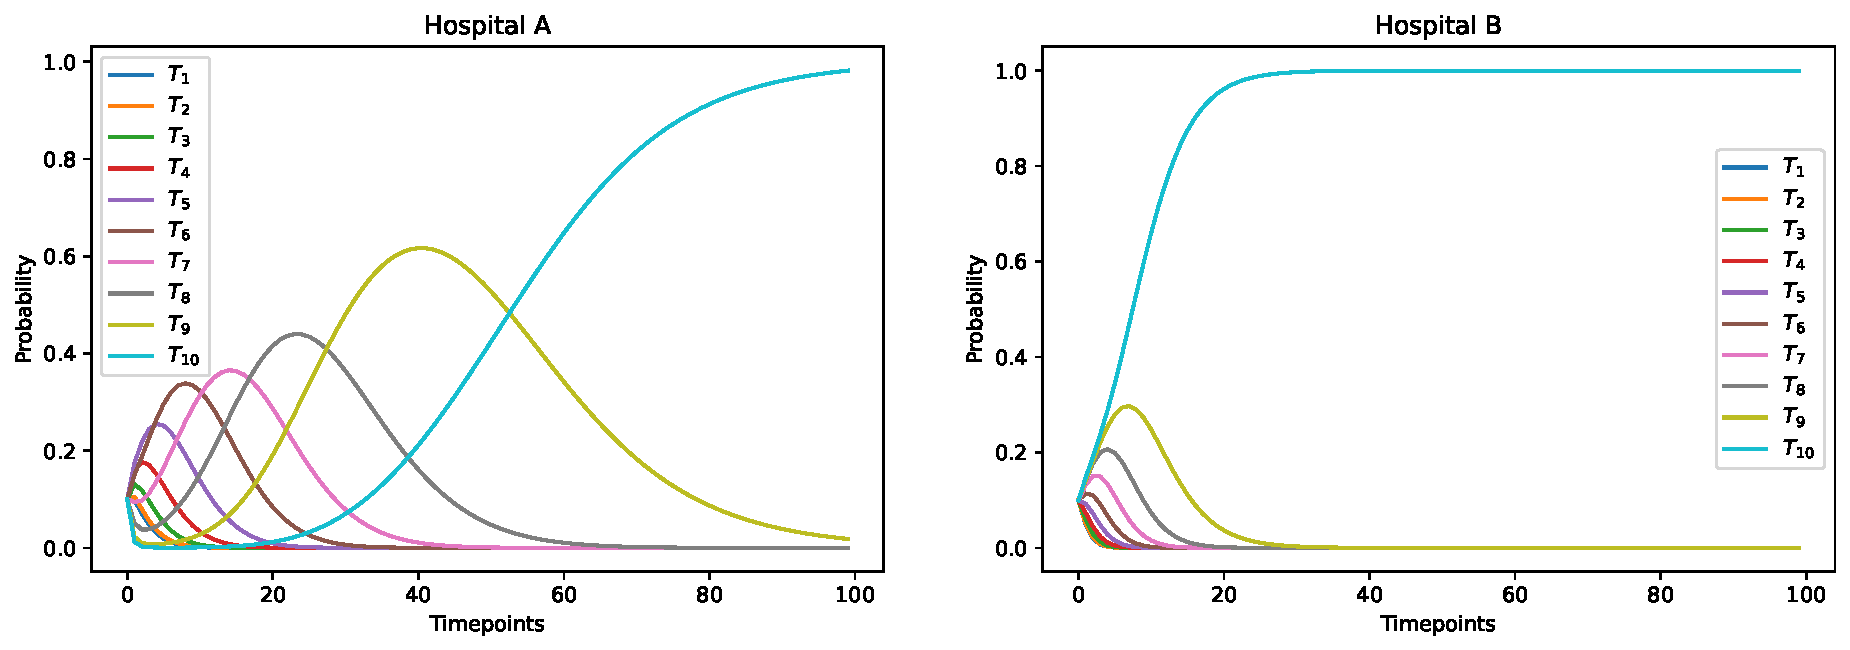
\includegraphics[width=\linewidth]{chapters/05_numerical_results/Bin/example_1/base_case.pdf}
    \caption{Example 1: Asymmetric replicator dynamics}
    \label{fig:asymmetric_replicator_dynamics_example_1}
\end{figure}

What is more important in this example is how the two hospitals reached these
decisions which also highlights the importance of using a learning algorithm.
Hospital \(B\) is able to reach the final decision in a shorter amount of time
while  hospital \(A\) takes longer and goes through numerous strategies to get
there based on the strategy choices of hospital \(B\).
By observing the strategy choices of hospital \(A\) more closely, it can be seen
that it starts out by blocking all ambulances and then slowly starts to unblock
them.

Consider the utility function of the two players from
equation~(\ref{eq:utility_queueing_systems}):

\begin{equation*}
    U_{T^A, T_B}^i = 1 - \left( \hat{P} - P(W_i < t) \right)^2
    \qquad i \in {A, B}
\end{equation*}

where the hospitals' aim is to have a proportion of patients \(\hat{P}\)
within the target time \(t\).
The utility function attempts to get the difference between the actual
proportion of patients within the target time \(t\) and the target proportion
\(\hat{P}\) as close to zero as possible.

Thus, for the current example, the fact that two hospitals are
motivated to play a strategy of \(T^A = 10, T^B = 10\) means that the target
of \(\hat{P} = 0.95\) and \(t = 2\) is effortlessly achieved given the current
parameters.
Hospitals \(A\) and \(B\) are able to achieve a target of \(t = 2\) and do not
need to block ambulances unless they reach their maximum capacity.

What if the target time \(t\) was decreased from \(t = 2\) to \(t = 1.7\)?
Now, in order for the hospitals to be maximise their utility, \(95\%\) of
patients would need to receive treatment within \(1.7\) hours from their time
of arrival instead of \(2\) hours.
Using the Lemke-Howson algorithm, the following pure strategy Nash equilibrium
arises:

\begin{equation}
    \sigma^A = (0, 0, 1, 0, 0, 0, 0, 0, 0, 0), \quad
    \sigma^B = (0, 0, 0, 0, 1, 0, 0, 0, 0, 0)
\end{equation}

This corresponds to hospital \(A\) playing a strategy of \(T^A = 3\) and
hospital \(B\) playing a strategy of \(T^B = 5\).
This means that hospital \(A\) will only block ambulances when the number of
patients in hospital \(A\) reaches \(3\) and hospital \(B\) will only block
ambulances when the number of patients in hospital \(B\) reaches \(5\).
Now 
these strategies emerge.
Figure~\ref{fig:asymmetric_replicator_dynamics_example_1_what_if_1} shows the
results of the asymmetric replicator dynamics algorithm with the decreased
target time \(t = 1.7\).

\begin{figure}[H]
    \centering
    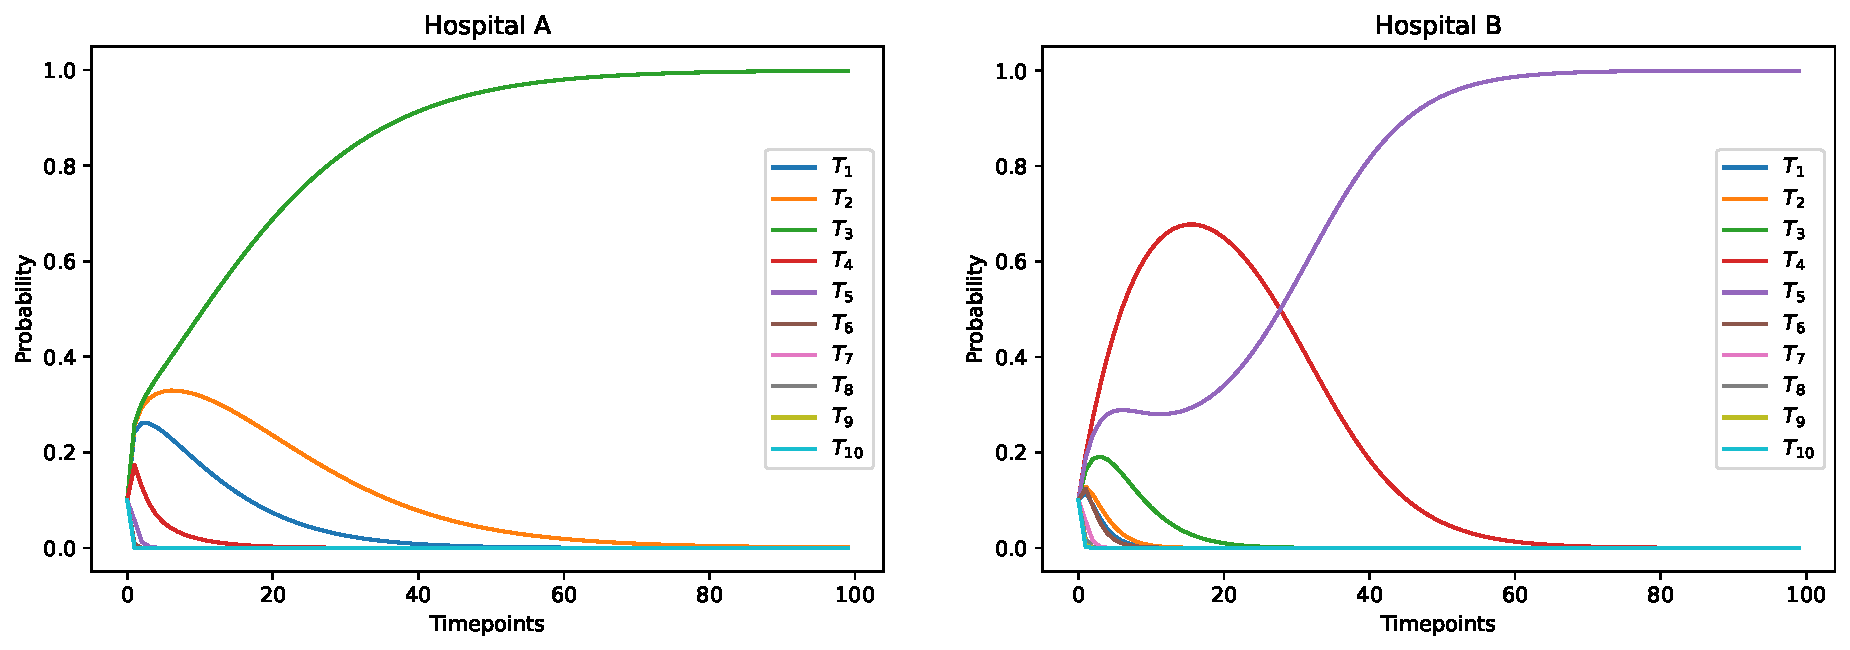
\includegraphics[width=\linewidth]{chapters/05_numerical_results/Bin/example_1/what_if_t_1.7.pdf}
    \caption{Example 1: Asymmetric replicator dynamics (what if \(t = 1.7\))}
    \label{fig:asymmetric_replicator_dynamics_example_1_what_if_1}
\end{figure}

It can be seen from
Figure~\ref{fig:asymmetric_replicator_dynamics_example_1_what_if_1} that the
two hospitals have reached the same output as the Lemke-Howson algorithm.
Hospital \(A\) chooses a strategy of \(T^A=3\) from a relatively early stage
while hospital \(B\) first starts playing a strategy of \(T^B=4\) and then
changes to \(T^B=5\) after a few iterations.
Therefore, given the results of the Lemke-Howson algorithm and the asymmetric
replicator dynamics algorithm, it can be seen that the more strict the time
target \(t\) is, the more hospitals would want to play a strategy where the
threshold is lower, and consequently, more ambulances will be blocked.

Additionally, the time target \(t\) can be decreased further to \(t = 1.5\).
Using the Lemke-Howson algorithm, the following pure strategy Nash equilibrium
arises:

\begin{equation}
    \sigma^A = (1, 0, 0, 0, 0, 0, 0, 0, 0, 0), \quad
    \sigma^B = (0, 1, 0, 0, 0, 0, 0, 0, 0, 0)
\end{equation}

This corresponds to hospital \(A\) playing a strategy of \(T^A = 1\) and
hospital \(B\) playing a strategy of \(T^B = 2\).
Now consider the equivalent asymmetric replicator dynamics algorithm run on
the modified example.

\begin{figure}[H]
    \centering
    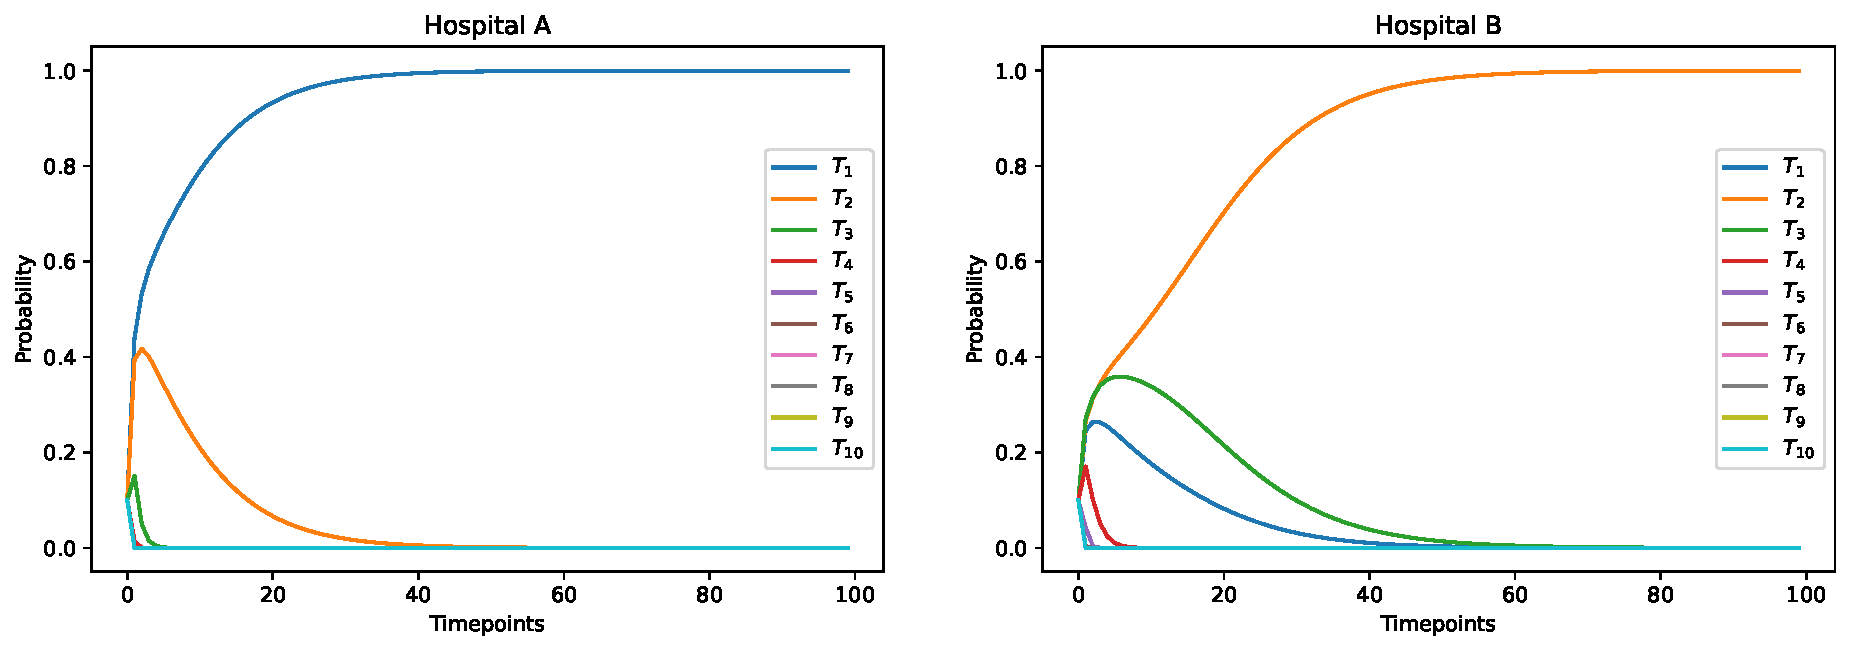
\includegraphics[width=\linewidth]{chapters/05_numerical_results/Bin/example_1/what_if_t_1.5.pdf}
    \caption{Example 1: Asymmetric replicator dynamics (what if \(t = 1.5\))}
    \label{fig:asymmetric_replicator_dynamics_example_1_what_if_2}
\end{figure}

It can be observed from
Figure~\ref{fig:asymmetric_replicator_dynamics_example_1_what_if_2} that the
two hospitals choose to play a strategy of \(T^A = 1\) and \(T^B = 2\).
This is the same as the pure strategy Nash equilibrium found using the
Lemke-Howson algorithm.
Therefore, it can be seen that by decreasing the time target \(t\) further,
hospitals tend to play a lower threshold strategy and consequently, more
ambulances will be blocked.

Table~\ref{tab:example_1_strategies_played_and_performance_measures} shows the
strategies played and the performance measures that arise from these strategy
choices for the three different time targets \(t = 2, 1.7, 1.5\).

\begin{table}[H]
    \centering
    \caption{Example 1: Strategies played and performance measures}
    \begin{tabular}{|c|ccc|ccc|}
        \hline
        Time target & \multicolumn{3}{c|}{Hospital A} &
        \multicolumn{3}{c|}{Hospital B} \\
        & Strategy & Waiting & Blocking & Strategy & Waiting & Blocking \\
        \hline
        \(t = 2\) & \(T = 10\) & 0.198 & 0.0006 & \(T = 10\) & 0.186 & 0.0006 \\
        \(t = 1.7\) & \(T = 3\) & 0.102 & 0.0904 & \(T = 5\) & 0.213 & 0.0894 \\
        \(t = 1.5\) & \(T = 1\) & 0.033 & 0.5852 & \(T = 2\) & 0.11 & 0.5592 \\
        \hline
    \end{tabular}
    \label{tab:example_1_strategies_played_and_performance_measures}
\end{table}

It can be seen from
Table~\ref{tab:example_1_strategies_played_and_performance_measures} that the
mean blocking time of ambulances increases as the time target \(t\) decreases.
Similarly, the mean waiting time of patients decreases as the time target \(t\)
decreases.
Note that for hospital \(B\) there is a slight increase of the mean waiting time
of patients when the time target \(t\) is decreased from \(t = 2\) to
\(t = 1.7\).
That is because of the strategy played by the third player; the EMS.
Observe the entries of the routing matrix \(R\) from
equation~(\ref{eq:results_payoff_matrices_1}).
The best response of the EMS when the hospital play \((T^A=10, T^B=10)\) is
to send a proportion of \(R_{10, 10} = 0.57\) patients to hospital \(A\)
while the best response of the EMS when the hospital play \((T^A=3, T^B=5)\)
is to send a proportion of \(R_{3, 5} = 0.45\) patients to hospital \(A\).
For that reason since hospital \(B\) receives more patients from the EMS when
the time target \(t\) is decreased from \(t = 2\) to \(t = 1.7\), the mean 
waiting time of patients increases slightly.


\subsection{Example 2}

Consider another example now where the parameters \(\lambda_2, \lambda_1^A
\lambda_1^B\) are set to a relatively high value.

\begin{multicols}{3}
    \begin{itemize}
        \item \( \lambda_1^A = 4.5 \)
        \item \( \mu^A = 2 \)
        \item \( C^A = 3 \)
        \item \( N^A = 6 \)
        \item \( M^A = 5 \)
        \columnbreak

        \item \( \lambda_1^B = 6 \)
        \item \( \mu^B = 3 \)
        \item \( C^B = 2 \)
        \item \( N^B = 7 \)
        \item \( M^B = 4 \)
        \columnbreak

        \item \( \lambda_2 = 10.7 \)
        \item \( t = 2 \)
        \item \( \alpha = 0.9 \)
        \item \( \hat{P} = 0.95 \)
    \end{itemize}
\end{multicols}

Recall that the relative traffic intensity of an \(M|M|c\) queue is given by
\(\rho = \frac{\lambda}{c \mu}\) where \(\lambda\) is the arrival rate, c is
the number of servers and \(\mu\) is the service rate.
The relative traffic intensity is a metric that measures how congested a queue
is, based on the inflow and outflow of individuals in the queue.
When \(\rho < 1\) the rate at which individuals leave the queue is larger than the rate at which
individuals enter
the queue and when \(\rho > 1\) the rate at which individuals enter the queue is larger
than that of those leaving the queue~\cite{almeida2018note}.

In this example, without solving the game, the relative traffic intensity of
each hospital cannot be calculated since the arrival rate of type 2 patients
among the two hospitals may vary based on the strategy played by the EMS.
Each hospital's relative traffic intensity is given by:

\begin{equation}
    \rho^A = \frac{\lambda_1^A + \lambda_2 p^A}{C^A \mu^A}, \qquad \qquad
    \rho^B = \frac{\lambda_1^B + \lambda_2 (1 - p^A)}{C^B \mu^B}, \qquad \qquad
    p^A \in [0, 1]
\end{equation}

where \(p^A\) is the proportion of type 2 patients that are sent to hospital
\(A\) by the EMS.
By substituting in all the values for the parameters, the relative traffic
intensity of each hospital is given by:

\begin{equation}
    \rho^A = \frac{4.5 + 10.7 p^A}{6}, \qquad \qquad
    \rho^B = \frac{16.7 - 10.7 p^A}{6}, \qquad \qquad
    p^A \in [0, 1]
\end{equation}

Thus, the traffic intensity of hospital \(A\) can take values \(\rho^A \in
[0.75, 2.53]\) while the traffic intensity of hospital \(B\) can take values
\(\rho^B \in [1, 2.78]\).
In fact the combined relative traffic intensity of the two hospitals is given
by:

\begin{equation}
    \rho^{A, B} = \rho^A + \rho^B = \frac{4.5 + 10.7 p^A}{6} +
    \frac{16.7 - 10.7 p^A}{6} = \frac{21.2}{6} = 3.53
\end{equation}

Any value of \(\rho^{A, B} > 2\) indicates that the combined inflow of the
two hospitals is higher than the combined outflow and in this case it is well
above \(2\).
Given these two highly congested hospitals, consider the game played by the
EMS and the two hospitals.
Note that for the presentation of these data an affine transformation has been
applied to the values of the payoff matrices to make it easier for the reader
(\(A_{ij} = 10000 (a_{ij} - 0.999) \text{ and }
B_{ij} = 10000 (b_{ij} - 0.999)\)).

\small
\begin{equation*}
    A = 
    \begin{bmatrix}
        5.0518 & 5.0518 & 5.0518 & 5.0518 & 5.0518 & 5.0518 & 5.0518 \\
        5.4989 & 5.4977 & 5.4960 & 5.4924 & 5.4844 & 5.4654 & 5.3875 \\
        6.8232 & 6.8192 & 6.8150 & 6.8065 & 6.7871 & 6.7334 & 6.4906 \\
        9.0298 & 9.0244 & 9.0187 & 9.0078 & 8.9827 & 8.9082 & 8.5145 \\
        9.9996 & 9.9994 & 9.9992 & 9.9987 & 9.9972 & 9.9893 & 9.8571 \\
        8.7740 & 8.8006 & 8.8249 & 8.8660 & 8.9438 & 9.1295 & 9.7157
    \end{bmatrix}
\end{equation*}

\begin{equation*}
    B = 
    \begin{bmatrix}
        1.7127 & 2.5822 & 4.6186 & 6.8497 & 8.9418 & 9.9999 & 8.2148 \\
        1.7127 & 2.5477 & 4.5634 & 6.8047 & 8.9150 & 9.9996 & 8.3358 \\
        1.7127 & 2.4528 & 4.3784 & 6.6441 & 8.8278 & 9.9965 & 8.5306 \\
        1.7127 & 2.4141 & 4.2867 & 6.5470 & 8.7656 & 9.9919 & 8.6745 \\
        1.7127 & 2.3415 & 4.0998 & 6.3265 & 8.6058 & 9.9716 & 8.9634 \\
        1.7127 & 2.1269 & 3.4930 & 5.4885 & 7.8353 & 9.7075 & 9.7322
    \end{bmatrix}
\end{equation*}

\begin{equation}
    R = 
    \begin{bmatrix}
        0.22 & 0.06 & 0.05 & 0.05 & 0.04 & 0.03 & 0.01 \\
        0.95 & 0.6  & 0.47 & 0.37 & 0.28 & 0.2  & 0.11 \\
        0.97 & 0.81 & 0.72 & 0.62 & 0.51 & 0.37 & 0.21 \\
        0.97 & 0.85 & 0.77 & 0.68 & 0.57 & 0.44 & 0.26 \\
        0.98 & 0.89 & 0.83 & 0.76 & 0.66 & 0.53 & 0.35 \\
        1.   & 0.95 & 0.91 & 0.87 & 0.8  & 0.7  & 0.52
    \end{bmatrix}
\end{equation}
\normalsize

Matrices \(A\) and \(B\) are the payoff matrices of the two hospitals and
can be used to get the Nash equilibrium of the game.
Using the Lemke-Howson algorithm, the following pure strategy Nash equilibrium
is found:

\begin{equation}
    \sigma^A = (0, 0, 0, 0, 1, 0), \quad
    \sigma^B = (0, 0, 0, 0, 0, 1, 0)
\end{equation}

The output of the Lemke-Howson algorithm indicates that the game is at a Nash
equilibrium when hospital \(A\) plays a strategy of \(T^A = 5\) and hospital
\(B\) plays a strategy of \(T^B = 6\).
In fact, this is the only Nash equilibrium of the game.
A similar outcome is obtained when using a learning algorithm.
Figure~\ref{fig:asymmetric_replicator_dynamics_example_2} shows the output of
the run of the asymmetric replicator dynamics algorithm.

\begin{figure}[H]
    \centering
    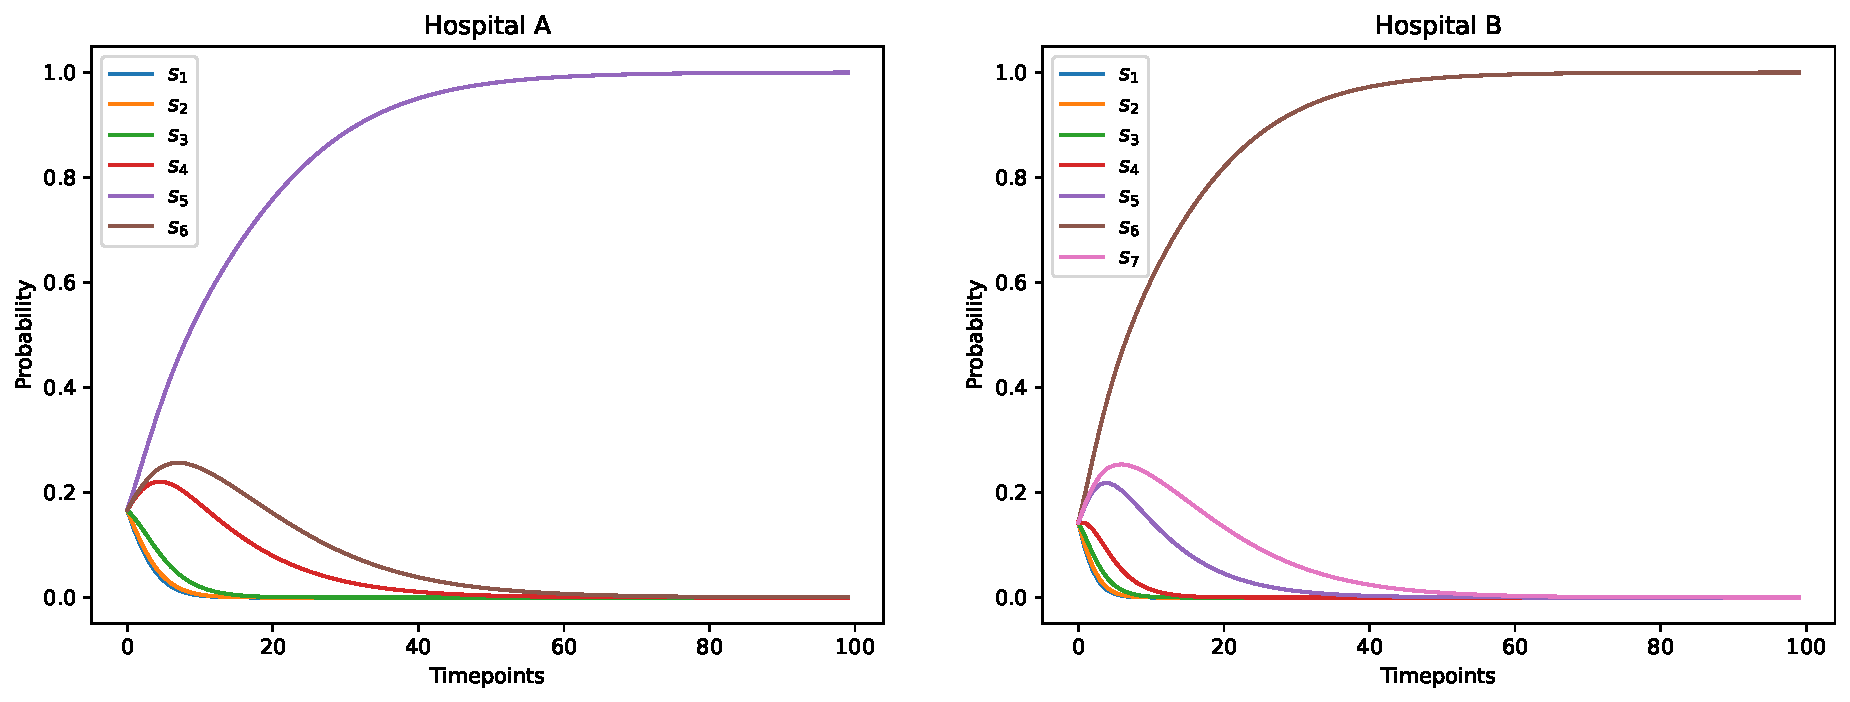
\includegraphics[width=\linewidth]{chapters/05_numerical_results/Bin/example_2/base_case.pdf}
    \caption{Example 2: Asymmetric replicator dynamics}
    \label{fig:asymmetric_replicator_dynamics_example_2}
\end{figure}

Asymmetric replicator dynamics converges to the same strategy as the Lemke-
Howson algorithm, which is the pair of strategies \((T^A = 5, T^B = 6)\).

Consider now the concept of the Price of Anarchy
(\(PoA\))~\cite{roughgarden2005selfish}.
\(PoA\) is a measure in game theory that is used to quantify the efficiency of
the outcome of a game when players behave in a selfish way.
Examples of using this measure in a healthcare setting include~\cite{} %  TODO Reference a few of my papers and others
More specifically, the \(PoA\) measures the ratio between the worst possible
equilibria outcome of a game (so that no players have an incentive to deviate) and the best possible centrally controlled outcome of the game (the best possible collective situation).
The \(PoA\) of a game is defined as:

\begin{equation}\label{eq:poa_definition}
    PoA = \frac{\max_{s \in E}{F(s)}}{\min_{s \in S}{F(s)}}
\end{equation}

where \(S\) is the set of all possible strategies of the players, \(E\) is the
set of all possible equilibria of the game and \(F(s)\) is a cost function to
measure the efficiency of when the players play strategy \(s\).
The \(PoA\) is a measure that is used to describe the overall efficiency of the
game, rather the independent efficiency of each player.

For the purpose of this study a measure is introduced that considers the
ratio between each hospital's best achievable blocking time and the one that is
being played.
This is defined as the compartmentalised price of anarchy of the
players of the game and is defined as \(PoA_i(s)\) where \(i \in \{A, B\}\) and
\(s \in S\) is the strategy played by player \(i\).
The compartmentalised price of anarchy is defined as:

\begin{equation}\label{eq:compartmentalised_poa_definition}
    PoA_i(s) = \frac{B_i(s)}{\min_{s' \in S}{B_i(s')}}
\end{equation}

That is the ratio between the blocking time of player \(i\) when playing the
chosen strategy \(s\) and the minimum blocking time player \(i\) could achieve
from any strategy \(s' \in S\).
In other words, the range of values that the compartmentalised \(PoA\) can take
are \(PoA_i(s) \in [1, +\infty)\), where \(1\) is the best possible outcome.
Consider, once again the asymmetric replicator dynamics run from
Figure~\ref{fig:asymmetric_replicator_dynamics_example_2}.
One may plot the compartmentalised \(PoA\) of each player alongside the outcome
of the learning algorithm.
Figure~\ref{fig:compartmentalised_poa_example_2} shows the asymmetric replicator
dynamics run of the game along with the compartmentalised \(PoA\) of each player.

\begin{figure}[H]
    \centering
    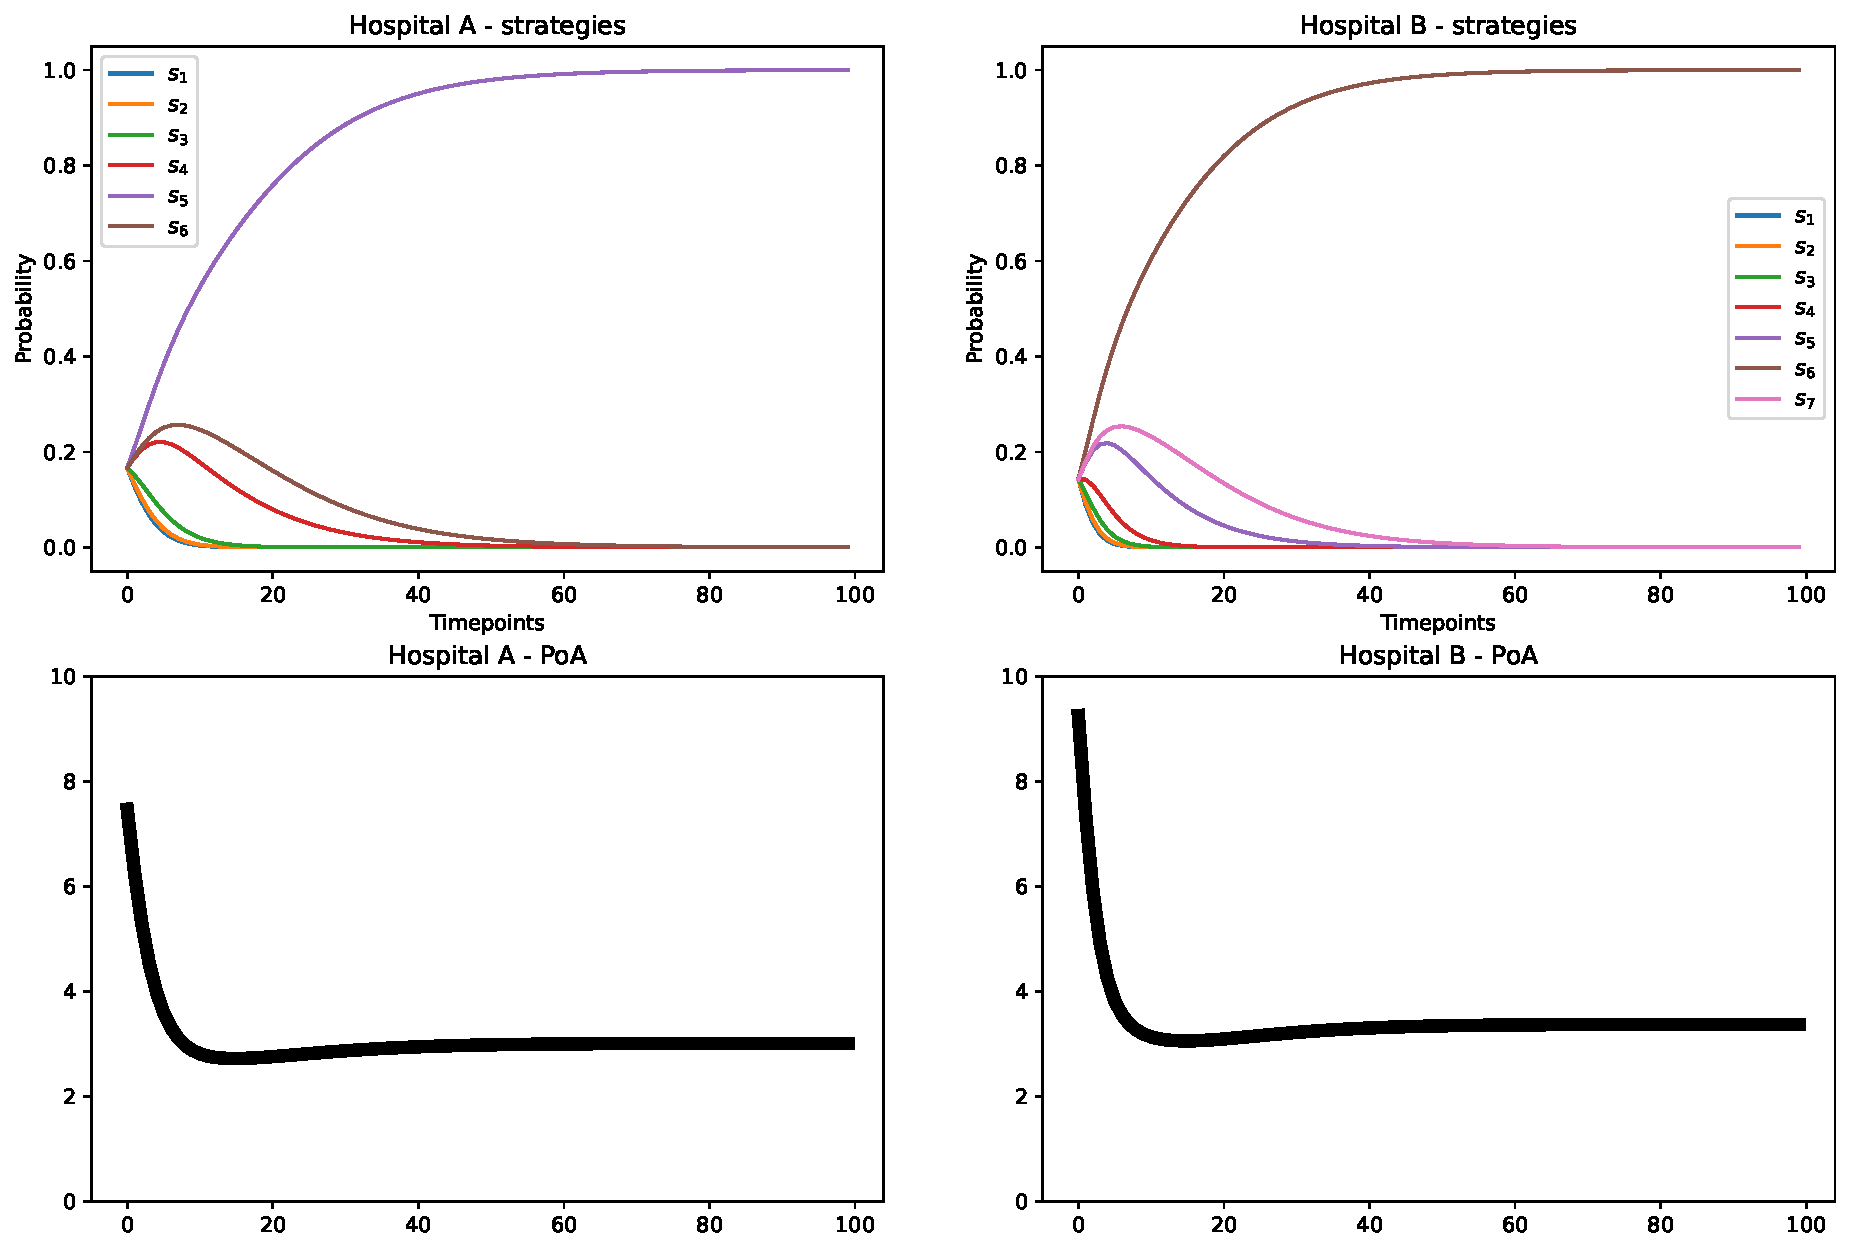
\includegraphics[width=\linewidth]{chapters/05_numerical_results/Bin/example_2/poa_ard_example_2.pdf}
    \caption{Example 2: Compartmentalised \(PoA\)}
    \label{fig:compartmentalised_poa_example_2}
\end{figure}

In Figure~\ref{fig:compartmentalised_poa_example_2} it can be seen that the
\(PoA\) of both players is always greater than \(1\).
This means that the chosen strategies are not the best possible strategies in
terms of minimising the blocking time of ambulances.
So, the question to be asked here is: what can be changed in the game to escape
these learned inefficiencies?

For the rest of this section, asymmetric replicator dynamics will be used in
a slightly different manner.
One could run asymmetric replicator dynamics on a modified version of the game
where certain parameters are changed and observe the outcome of the learning
algorithm.
Although this is a sensible approach, doing that means that the learned
strategies from Figure~\ref{fig:compartmentalised_poa_example_2} are not
considered.
As mentioned earlier, the aim is to investigate how to escape these learned
inefficiencies, not what would happen if they never existed.
Therefore, a different approach is considered.
Learning algorithms require only matrices \(A\) and \(B\) to run.
Therefore, asymmetric replicator dynamics is ran on the original game and
stopped at a certain point.
After changing the parameters of the game, the new matrices arise, \(\tilde{A}\)
and \(\tilde{B}\).
Asymmetric replicator dynamics is then ran again on the new matrices while
using the final strategies from the previous run as the initial strategies.
This approach is used to investigate how the strategies and the \(PoA\) of
the players change when the values of the parameters change.

One sensible idea would be to increase the artificial values of the hospital
capacities \(N^i\).
The same learning algorithm is ran again with the same parameters as before, but
at some point the artificial values are increased from \(N^A = 6\) and
\(N^B = 7\) to \(N^A = 7\) and \(N^B = 8\).
Figure~\ref{fig:poa_ard_example_2_system_capacity} shows the output of the
asymmetric replicator dynamics algorithm and the compartmentalised \(PoA\) of
each player.
Note that, when the artificial values are increased, hospital \(A\) gets a new
strategy of \(T^A = 7\) and hospital \(B\) gets a new strategy of \(T^B = 8\). 

\begin{figure}[H]
    \centering
    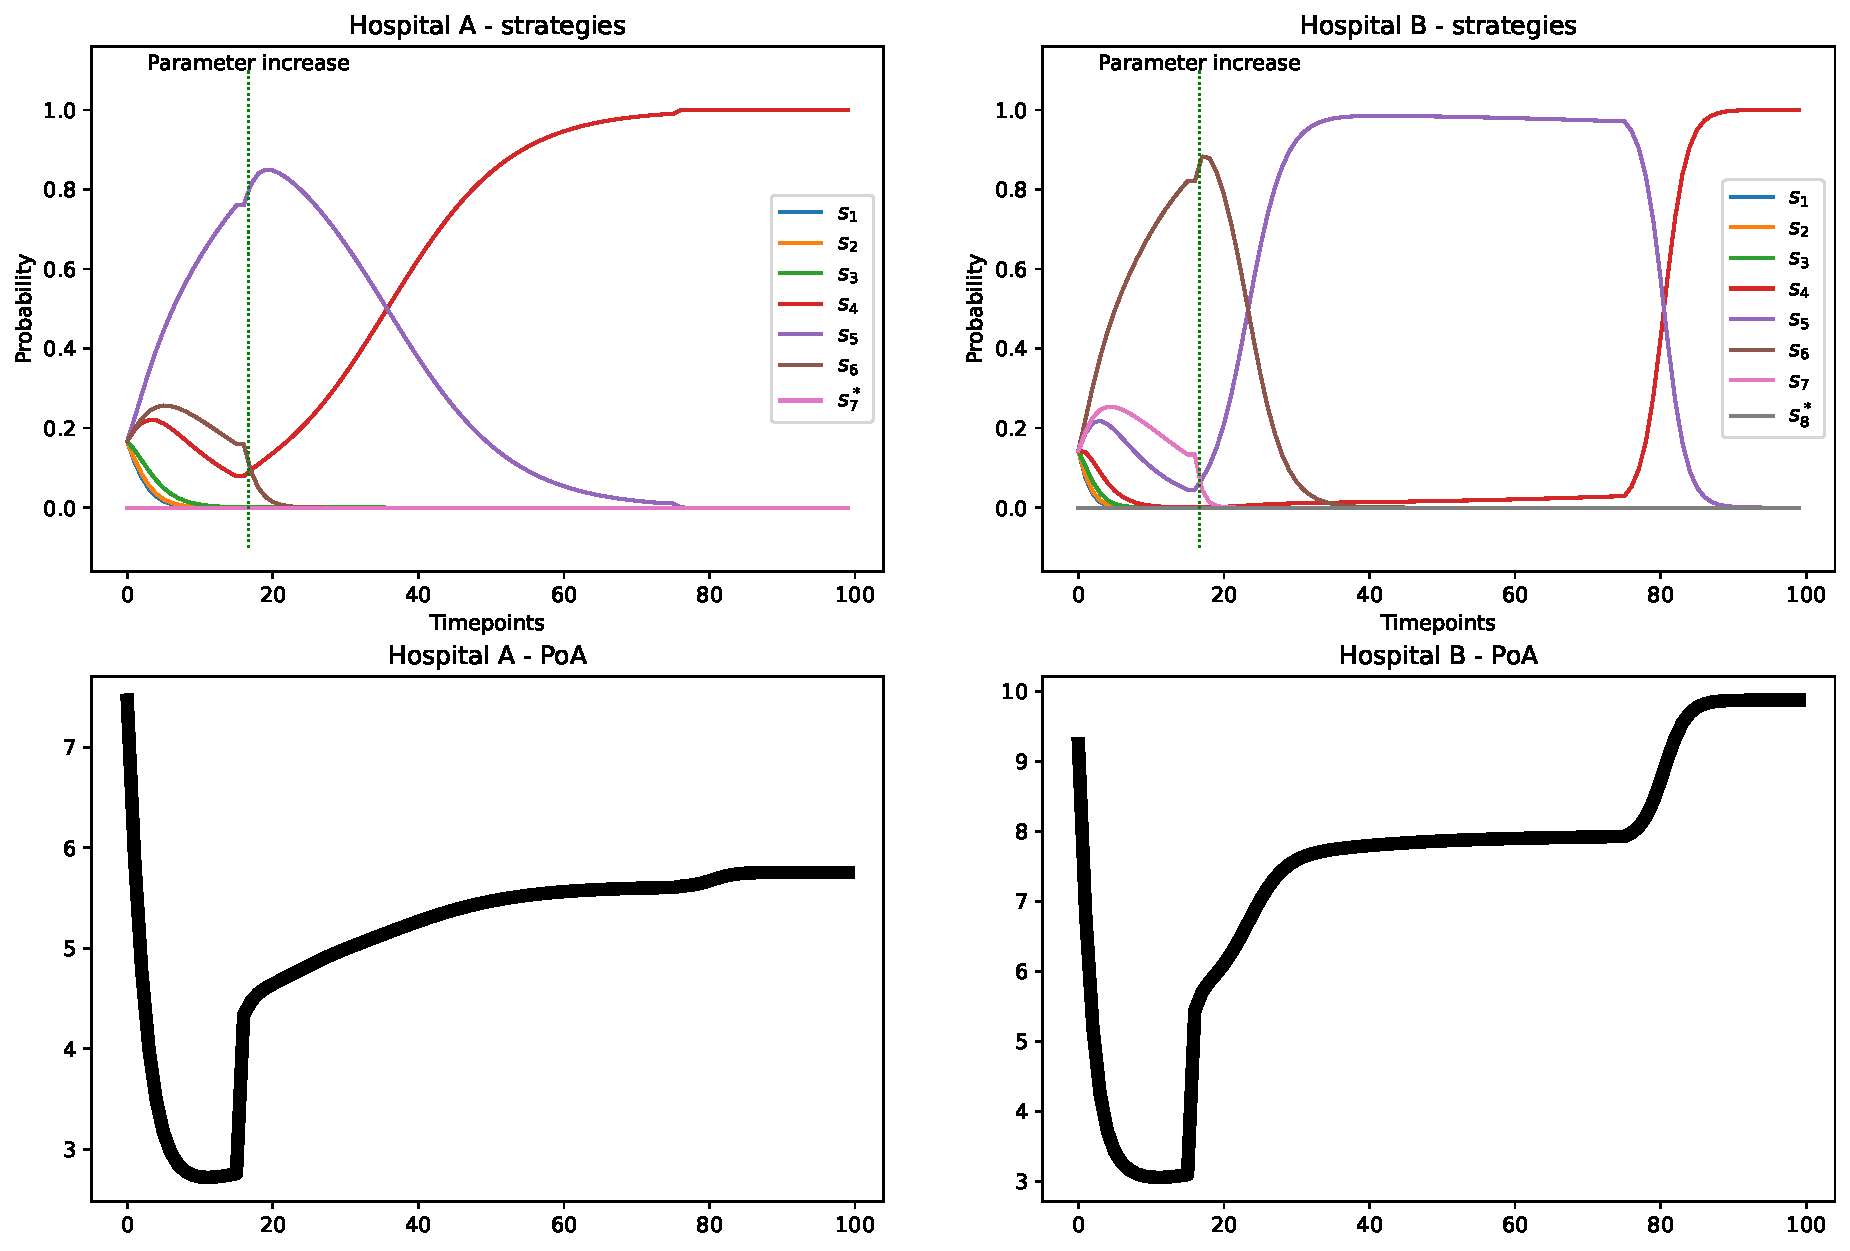
\includegraphics[width=\linewidth]{chapters/05_numerical_results/Bin/example_2/poa_ard_example_2_hospital_space.pdf}
    \caption{Example 2: Asymmetric replicator dynamics and compartmentalised
    \(PoA\) with increased hospital capacity \(N\)}
    \label{fig:poa_ard_example_2_system_capacity}
\end{figure}

In fact, by increasing the capacity of the hospitals, both hospitals become
even more inefficient.
The moment the capacities are increased, both hospitals change their strategies
to close their doors for ambulance patients even earlier.
That causes the blocking time of ambulances to increase and thus the \(PoA\) of
both players increase.
This happens because there are so many individuals coming in that the hospitals
cannot cope with the demand.

Similarly, the same learning algorithm is ran again with the same parameters as
before, but at some point the parking capacity of the hospitals is increased
from \(M^A = 5\) and \(M^B = 4\) to \(M^A = 20\) and \(M^B = 16\).
Figure~\ref{fig:poa_ard_example_2_parking_capacity} shows the output of the
asymmetric replicator dynamics algorithm and the compartmentalised \(PoA\) of
each player.

\begin{figure}[H]
    \centering
    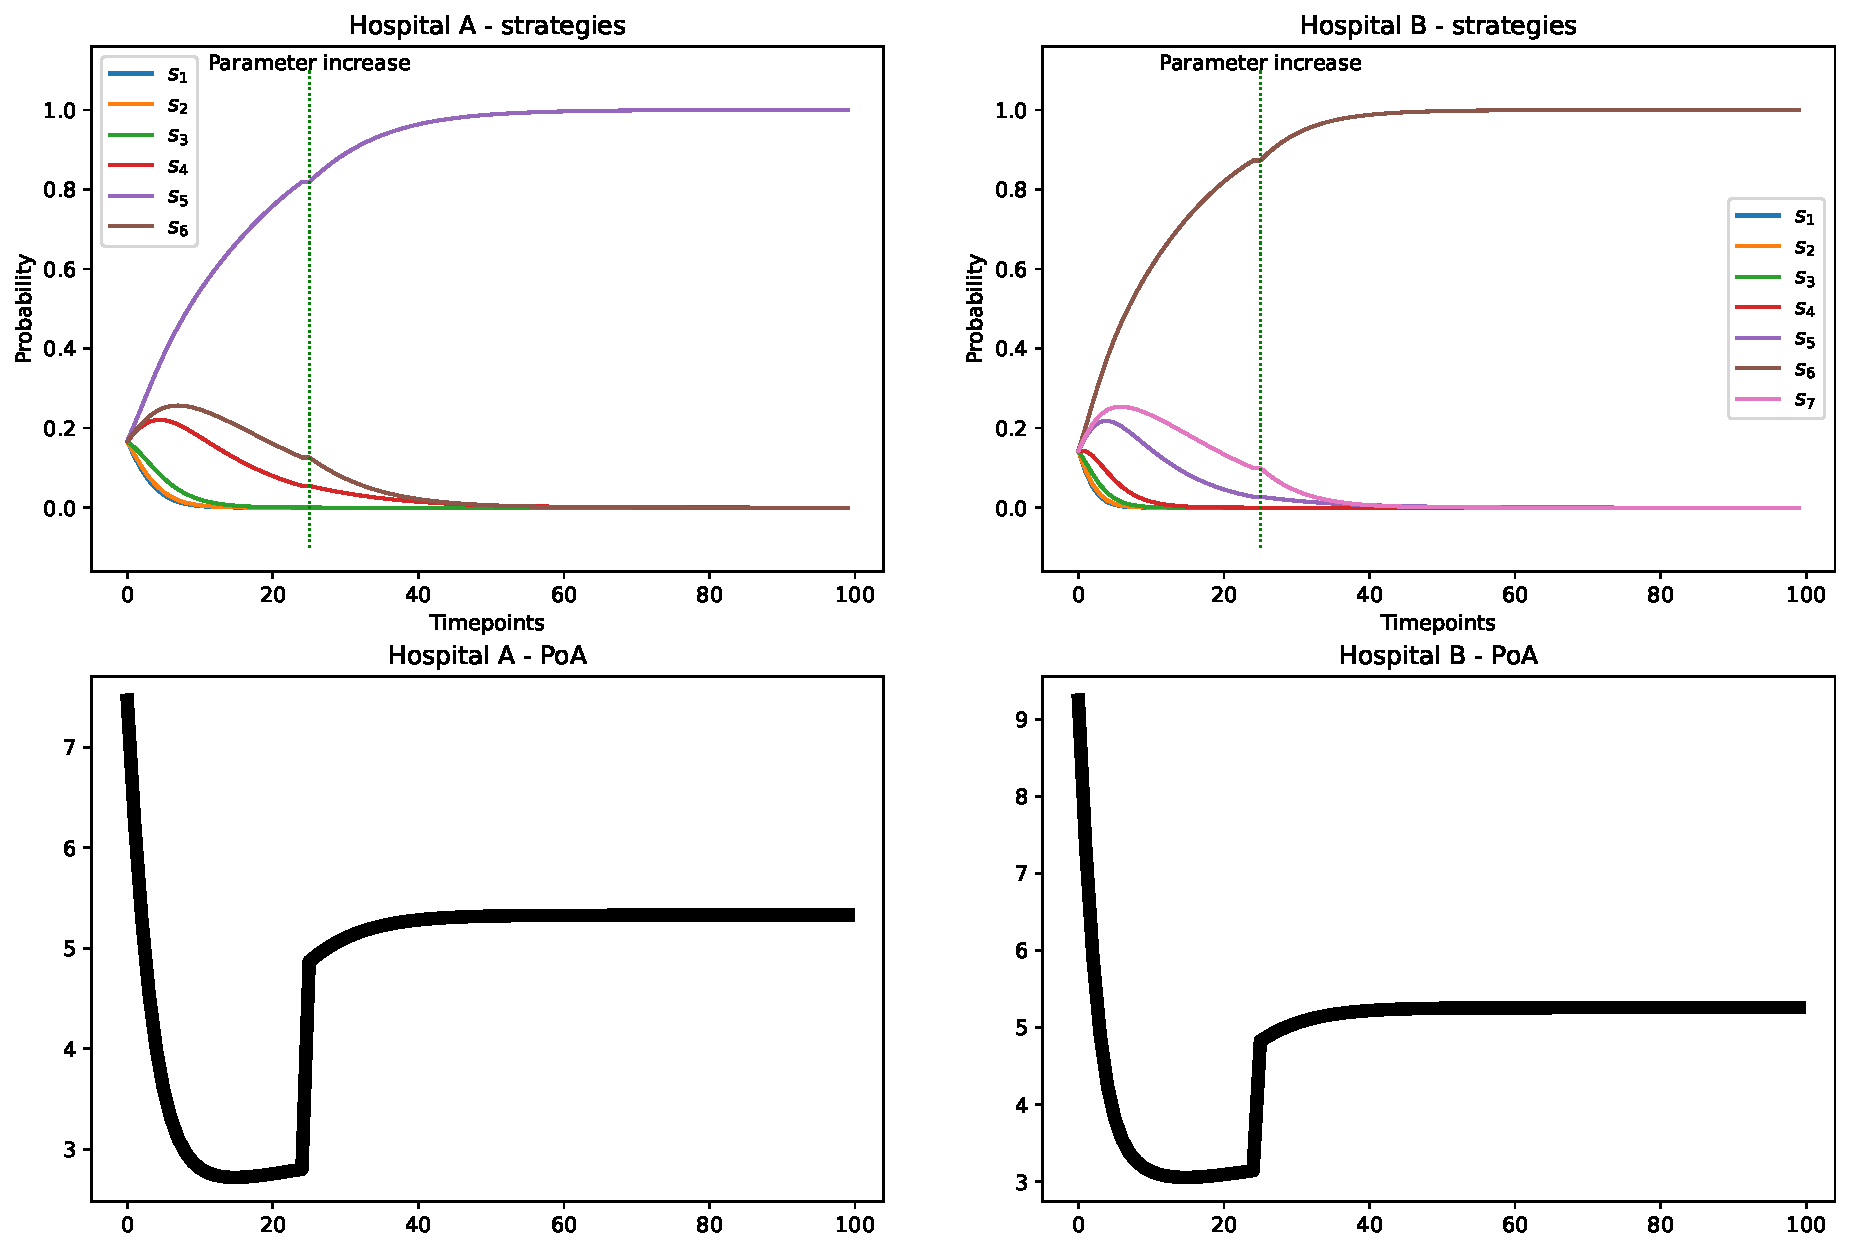
\includegraphics[width=\linewidth]{chapters/05_numerical_results/Bin/example_2/poa_ard_example_2_parking_space.pdf}
    \caption{Example 2: Asymmetric replicator dynamics and compartmentalised
    \(PoA\) with increased parking capacity \(M\)}
    \label{fig:poa_ard_example_2_parking_capacity}
\end{figure}

Although this time the strategies do not change, the \(PoA\) of both players
increases, which makes the entire game more inefficient in terms of the
blocking time of ambulances.
This is because the parking capacity of the hospitals is increased, which means
that patients can now wait longer in the parking space.
Therefore, the \(PoA\) gets worse because the blocking time of ambulances
when playing strategies \(T^A = 5\) and \(T^B = 6\) is increased.

Figures~\ref{fig:poa_ard_example_2_parking_capacity} and
\ref{fig:poa_ard_example_2_system_capacity} demonstrate how when increasing
the hospital capacities or the parking capacities make the outcome of the game
even more inefficient.
Consider now the case that the arrival rate of type 2 individuals \(\lambda_2\)
is increased at some point during the learning algorithm.
Similar to before, the learning algorithm is ran with the initial parameters,
and then \(\lambda_2\) is increased.
Figure~\ref{fig:poa_ard_example_2_lambda_2} shows the output of the asymmetric
replicator dynamics algorithm and the compartmentalised \(PoA\) of each player.

\begin{figure}[H]
    \centering
    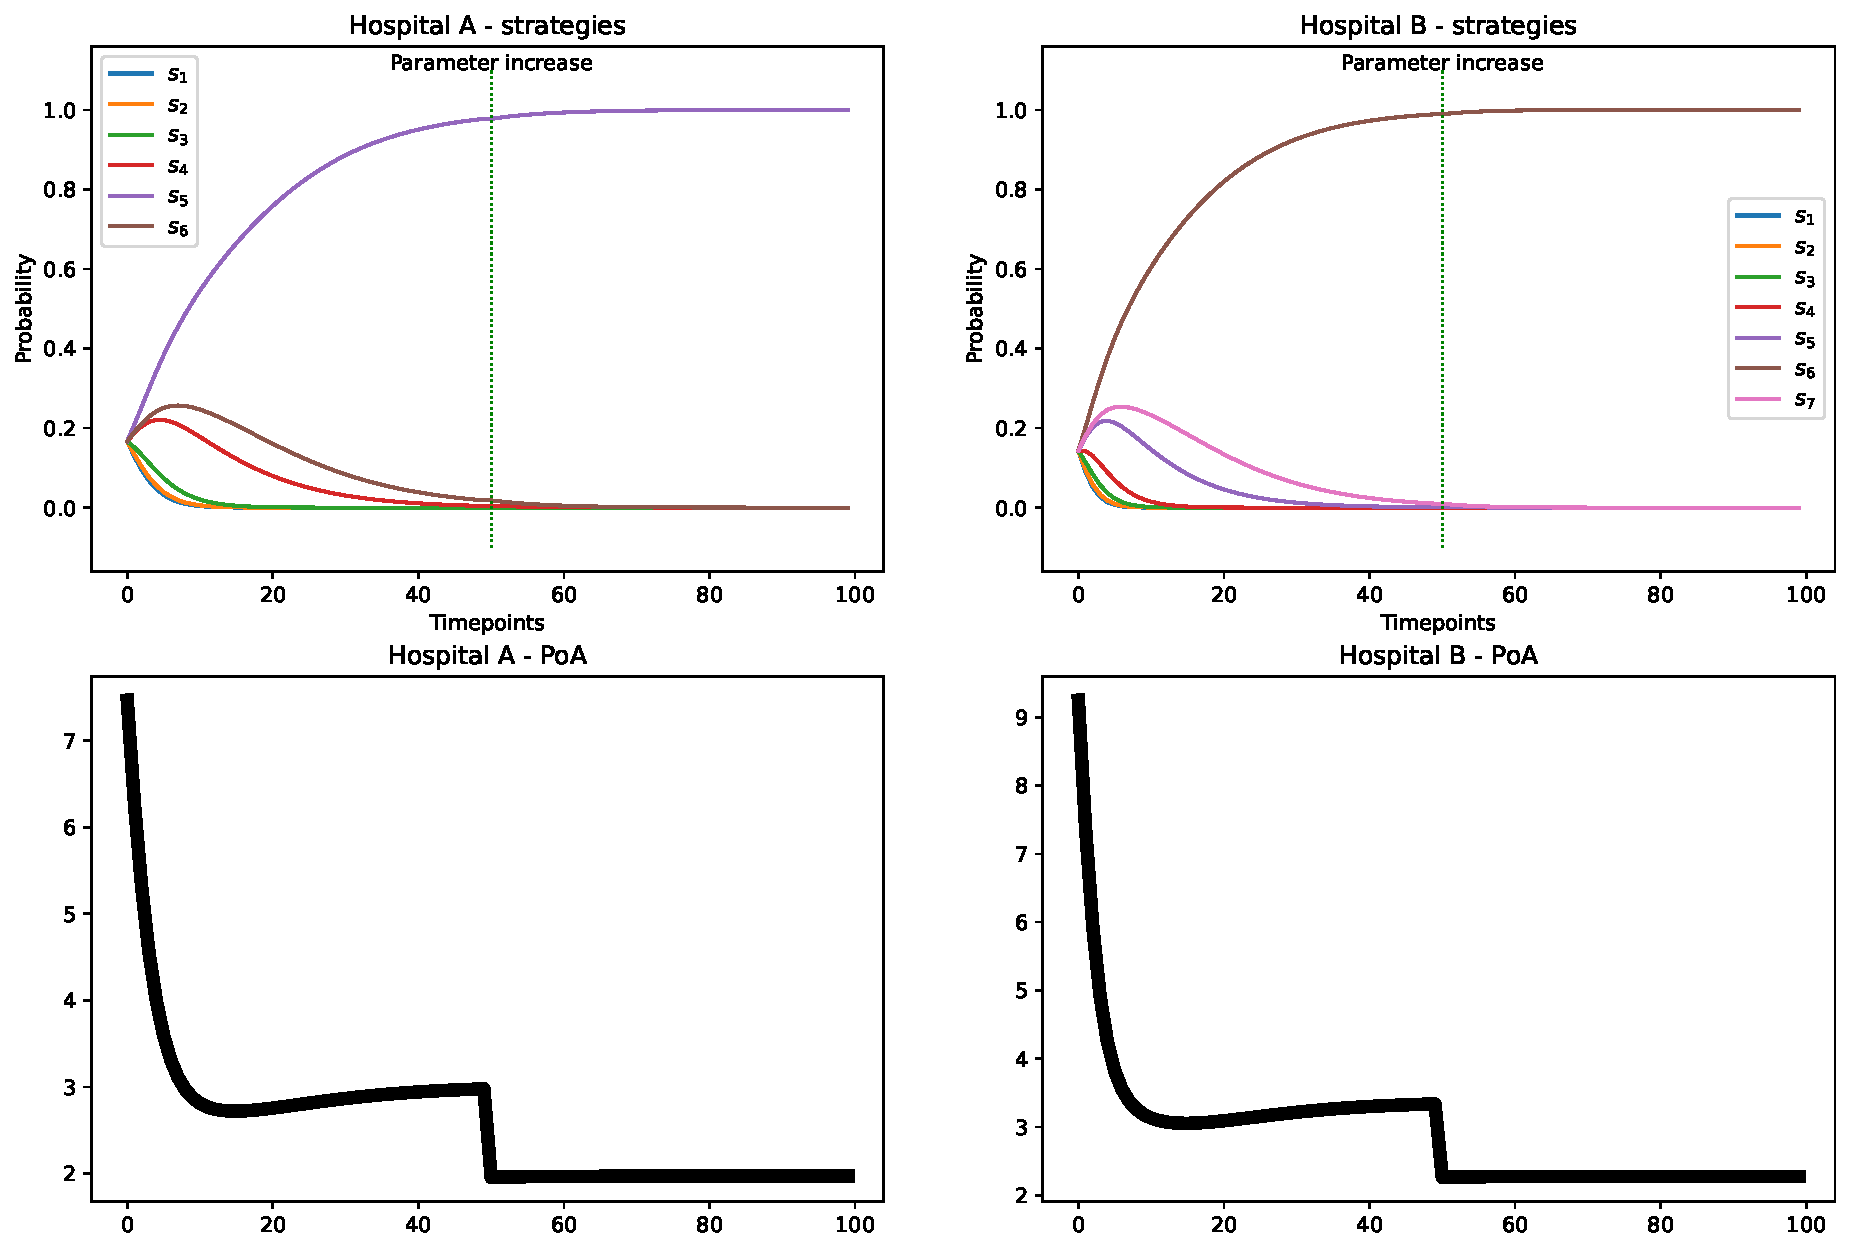
\includegraphics[width=\linewidth]{chapters/05_numerical_results/Bin/example_2/poa_ard_example_2_lambda_2.pdf}
    \caption{Example 2: Asymmetric replicator dynamics and compartmentalised
    \(PoA\) with increased arrival of type 2 patients \(\lambda_2\)}
    \label{fig:poa_ard_example_2_lambda_2}
\end{figure}

While the strategies of the players don't change, the \(PoA\) of both players
actually decreases.
Increasing the arrival rate of type 2 patients (ambulance patients) shouldn't
make the game more efficient, but it does.
That is not because the blocking time is decreased.
As a matter of fact the blocking time of ambulances increases for both players.
The reason why the \(PoA\) decreases can be traced back to the definition of the
\(PoA\) from equation~\ref{eq:compartmentalised_poa_definition}.
\(PoA_i(s)\) is defined as ratio between the blocking time when strategy \(s\)
is played and the best achievable blocking time from all strategies.
Therefore, when the best achievable blocking time becomes worse, the \(PoA\) of
the players decreases, which is exactly what happens in this case.
Although this is an interesting outcome, it is not a sensible one.
Increasing the arrival rate of an already flooded system does not make the
system more efficient.

A more appropriate way to increase the efficiency of the system is to increase
the number of staff \(C\).
Figure~\ref{fig:poa_ard_example_2_num_of_servers} shows the output of the
asymmetric replicator dynamics algorithm and the compartmentalised \(PoA\) of
each player when the number of staff available is increased from \(C^A = 3\)
and \(C^B = 2\) to \(C^A = 4\) and \(C^B = 3\).

\begin{figure}[H]
    \centering
    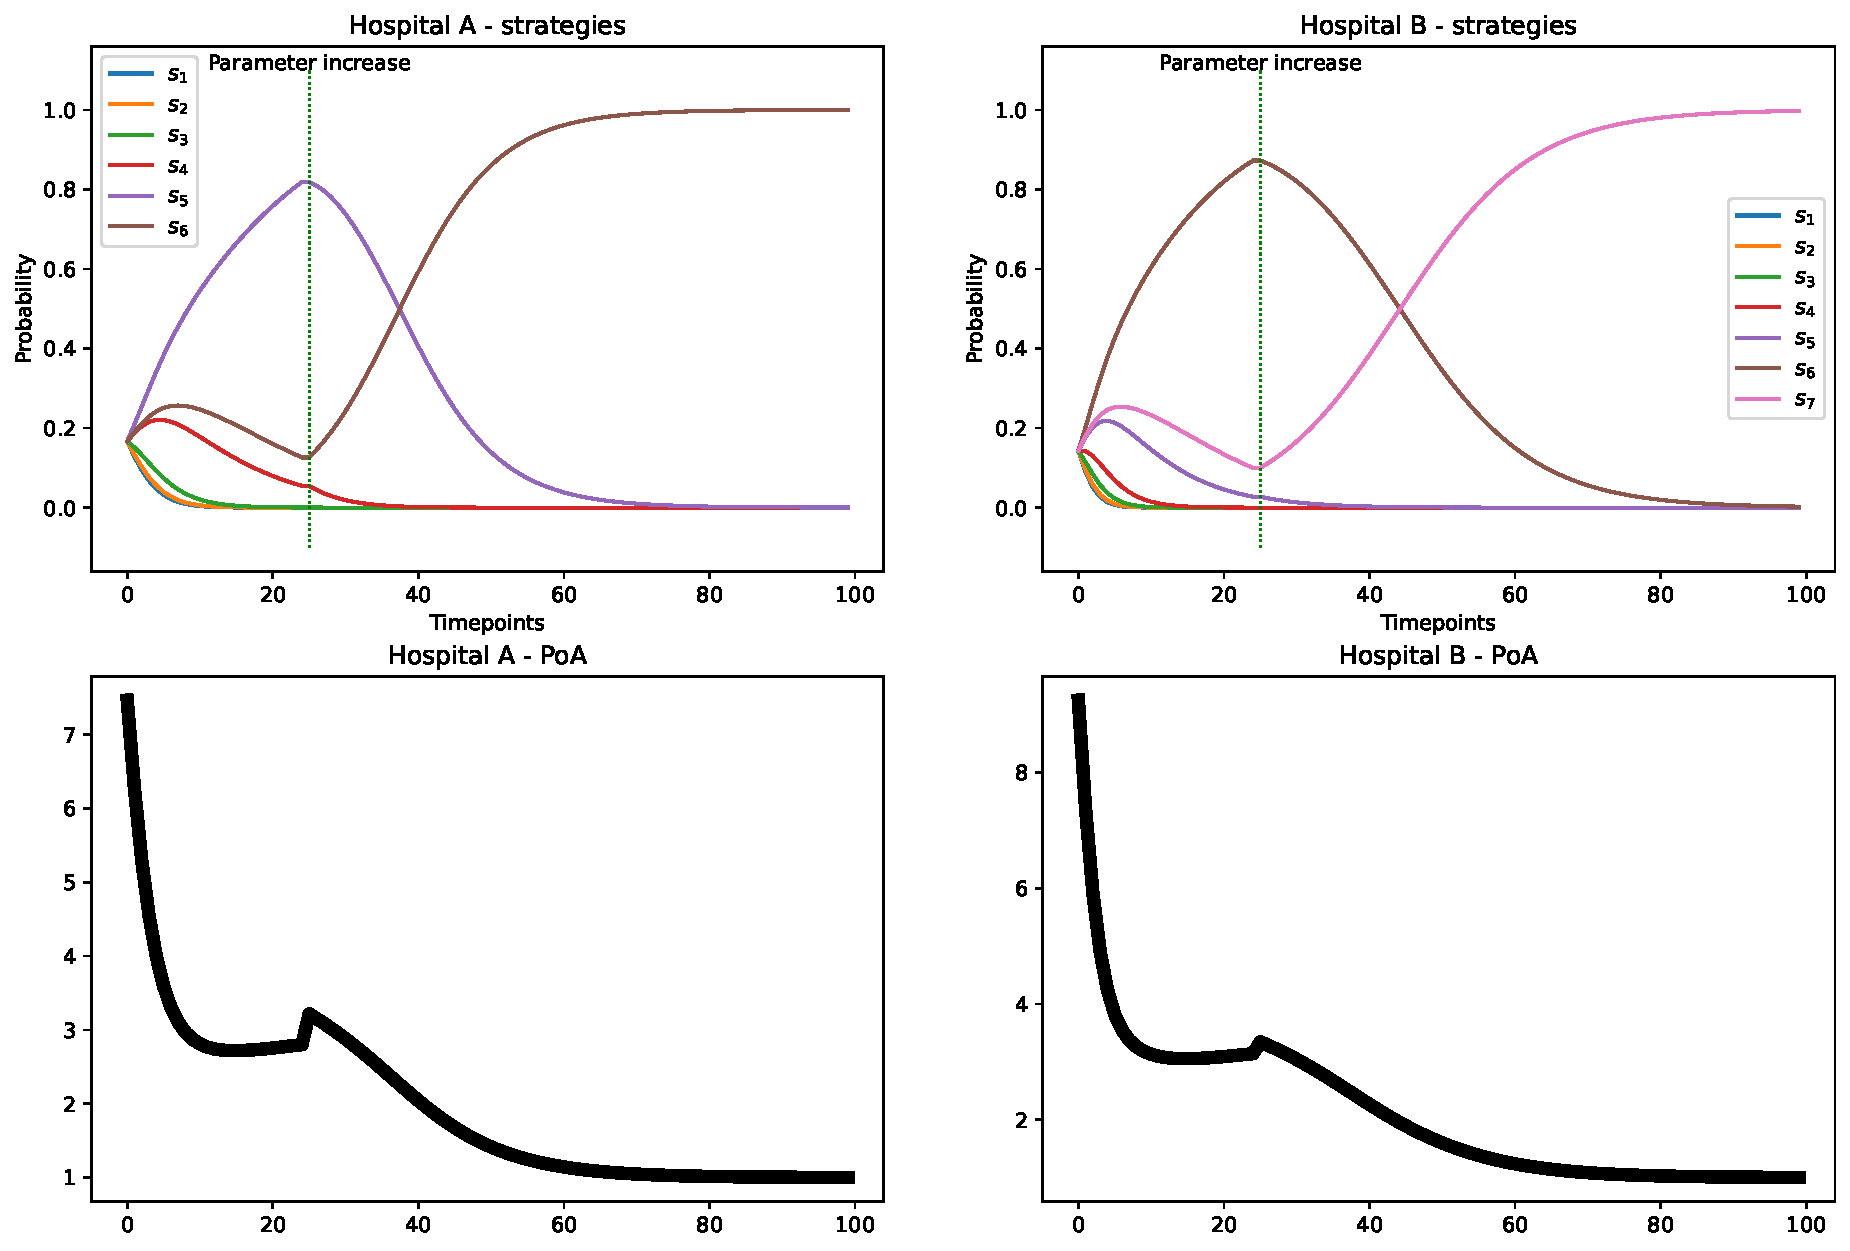
\includegraphics[width=\linewidth]{chapters/05_numerical_results/Bin/example_2/poa_ard_example_2_num_of_servers.pdf}
    \caption{Example 2: Asymmetric replicator dynamics and compartmentalised
    \(PoA\) with increased number of staff \(C\)}
    \label{fig:poa_ard_example_2_num_of_servers}
\end{figure}

Not only do the strategies of both players change, but the \(PoA\) of both
players also decreases.
Strategies \(T^A = 5\) and \(T^B = 6\) are no longer the strategies that are
played.
Instead, players play strategies \(T^A = 6\) and \(T^B = 7\), which makes the
hospitals accept more patient from ambulances, which in turn decreases the
mean blocking time of ambulances.
As a result the \(PoA\) decrease for both players indicating that the game has
reached a more efficient outcome in terms of the overall blocking time.

Although, Figure~\ref{fig:poa_ard_example_2_num_of_servers} shows a valid
way to increase the efficiency of the system, it might not be the most
cost-effective method, since more staff means more costs.
Another attempt to increase the efficiency of the system is to apply certain
incentives to the players to change their strategies.
The outcomes of the asymmetric replicator dynamics algorithm are derived
directly from matrices \(A\) and \(B\).
Therefore by carefully altering the values of these matrices, the strategies of
the players can be changed.
In other words, by penalising the chosen strategies the players could be forced
to play different ones.
For instance, consider the following example of matrices \(A\) and \(B\):

\begin{equation}
    A = 
    \begin{pmatrix}
        a_{11} & a_{12} & a_{13} & a_{14} \\
        a_{21} & a_{22} & a_{23} & a_{24} \\
        a_{31} & a_{32} & a_{33} & a_{34} \\    
    \end{pmatrix}, \quad
    B = 
    \begin{pmatrix}
        b_{11} & b_{12} & b_{13} & b_{14} \\
        b_{21} & b_{22} & b_{23} & b_{24} \\
        b_{31} & b_{32} & b_{33} & b_{34} \\    
    \end{pmatrix}
\end{equation}

These matrices now form a game that can be solved using the asymmetric
replicator dynamics algorithm.
In addition, these matrices can also be altered so that certain strategies are
penalised.
Strategies for player \(A\) are represented by rows of matrix \(A\), and
strategies for player \(B\) are represented by columns of matrix \(B\).
Therefore, an entire row of matrix \(A\) can be multiplied by a certain
constant \(p \in [0, 1]\) to penalise a strategy of player \(A\) and an entire
column of matrix \(B\) can be multiplied by the same factor to penalise a
strategy of player \(B\).
The resulting two matrices are denoted by \(\tilde{A}\) and \(\tilde{B}\) and
have certain strategies 

\begin{equation}
    A = 
    \begin{pmatrix}
        a_{11}   & a_{12}   & a_{13}   & a_{14}   \\
        p a_{21} & p a_{22} & p a_{23} & p a_{24} \\
        a_{31}   & a_{32}   & a_{33}   & a_{34}   \\    
    \end{pmatrix}, \quad
    B = 
    \begin{pmatrix}
        b_{11} & p b_{12} & b_{13} & b_{14} \\
        b_{21} & p b_{22} & b_{23} & b_{24} \\
        b_{31} & p b_{32} & b_{33} & b_{34} \\    
    \end{pmatrix}
\end{equation}

Therefore consider the payoff matrices of the two hospitals \(A\) and \(B\)
with the played strategies highlighted.


\begin{equation*}
    A = 
    \begin{bmatrix}
        5.0518 & 5.0518 & 5.0518 & 5.0518 & 5.0518 &
        5.0518 & 5.0518 \\
        5.4989 & 5.4977 & 5.4960 & 5.4924 & 5.4844 &
        5.4654 & 5.3875 \\
        6.8232  & 6.8192 & 6.8150 & 6.8065 & 6.7871  &
        6.7334 & 6.4906 \\
        9.0298 & 9.0244 & 9.0187 & 9.0078 & 8.9827 &
        8.9082 & 8.5145 \\
        \color{blue}{9.9996} & \color{blue}{9.9994} & \color{blue}{9.9992} & 
        \color{blue}{9.9987} & \color{blue}{9.9972} & \color{blue}{9.9893} & 
        \color{blue}{9.8571} \\
        8.7740 & 8.8006 & 8.8249 & 8.8660 & 8.9438 &
        9.1295 & 9.7157
    \end{bmatrix}
\end{equation*}

\begin{equation*}
    B = 
    \begin{bmatrix}
        1.7127 & 2.5822 & 4.6186 & 6.8497 & 8.9418 &
        \color{red}{9.9999} & 8.2148 \\
        1.7127 & 2.5477 & 4.5634 & 6.8047 & 8.9150  &
        \color{red}{9.9996} & 8.3358 \\
        1.7127 & 2.4528    & 4.3784 & 6.6441 & 8.8278 &
        \color{red}{9.9965} & 8.5306 \\
        1.7127 & 2.4141 & 4.2867 & 6.5470 & 8.7656 &
        \color{red}{9.9919} & 8.6745 \\
        1.7127 & 2.3415 & 4.0998 & 6.3265 & 8.6058 &
        \color{red}{9.9716} & 8.9634 \\
        1.7127 & 2.1269 & 3.4930 & 5.4885 & 7.8353 &
        \color{red}{9.7075} & 9.7322 \\
    \end{bmatrix}
\end{equation*}

Hospital \(A\) plays a strategy of \(T^A = 5\) and hospital \(B\) plays a
strategy of \(T^B = 6\).
By applying a penalty to the strategies of \(T^A = 5\) and \(T^B = 6\), the
resulting payoff matrices \(\tilde{A}\) and \(\tilde{B}\) are as follows.

\begin{equation*}
    \tilde{A} = 
    \begin{bmatrix}
        5.0518 & 5.0518 & 5.0518 & 5.0518 & 5.0518 &
        5.0518 & 5.0518  \\
        5.4989 & 5.4977 & 5.4960 & 5.4924 & 5.4844 &
        5.4654 & 5.3875 \\
        6.8232 & 6.8192 & 6.8150 & 6.8065 & 6.7871 &
        6.7334 & 6.4906 \\
        9.0298 & 9.0244 & 9.0187 & 9.0078 & 8.9827 &
        8.9082 & 8.5145 \\
        \color{blue}{6.9996} & \color{blue}{6.9994} & \color{blue}{6.9992} &
        \color{blue}{6.9987} & \color{blue}{6.9972} & \color{blue}{6.9893} &
        \color{blue}{6.8571} \\
        8.7740 & 8.8006 & 8.8249 & 8.8660 & 8.9438 &
        9.1295 & 9.7157 \\
    \end{bmatrix}
\end{equation*}


\begin{equation*}
    \tilde{B} = 
    \begin{bmatrix}
        1.7127 & 2.5822 & 4.6186 & 6.8497 & 8.9418 &
        \color{red}{6.9999} & 8.2148 \\
        1.7127 & 2.5477 & 4.5634 & 6.8047 & 8.9150 &
        \color{red}{6.9996} & 8.3358 \\
        1.7127 & 2.4528   & 4.3784 & 6.6441 & 8.8278 &
        \color{red}{6.9965} & 8.5306 \\
        1.7127 & 2.4141 & 4.2867 & 6.5470 & 8.7656 &
        \color{red}{6.9919} & 8.6745 \\
        1.7127 & 2.3415 & 4.0998 & 6.3265 & 8.6058 &
        \color{red}{6.9716} & 8.9634  \\
        1.7127 & 2.1269 & 3.4930 & 5.4885 & 7.8353 &
        \color{red}{6.7076} & 9.7322 \\
    \end{bmatrix}
\end{equation*}

Having penalised the strategies of \(T^A = 5\) and \(T^B = 6\),
Figure~\ref{fig:poa_ard_example_2_penalty} shows the outcome of asymmetric
replicator dynamics when initialising the algorithm with the initial matrices
\(A\) and \(B\) and at some point replacing them with the penalised ones
\(\tilde{A}\) and \(\tilde{B}\). 

\begin{figure}[H]
    \centering
    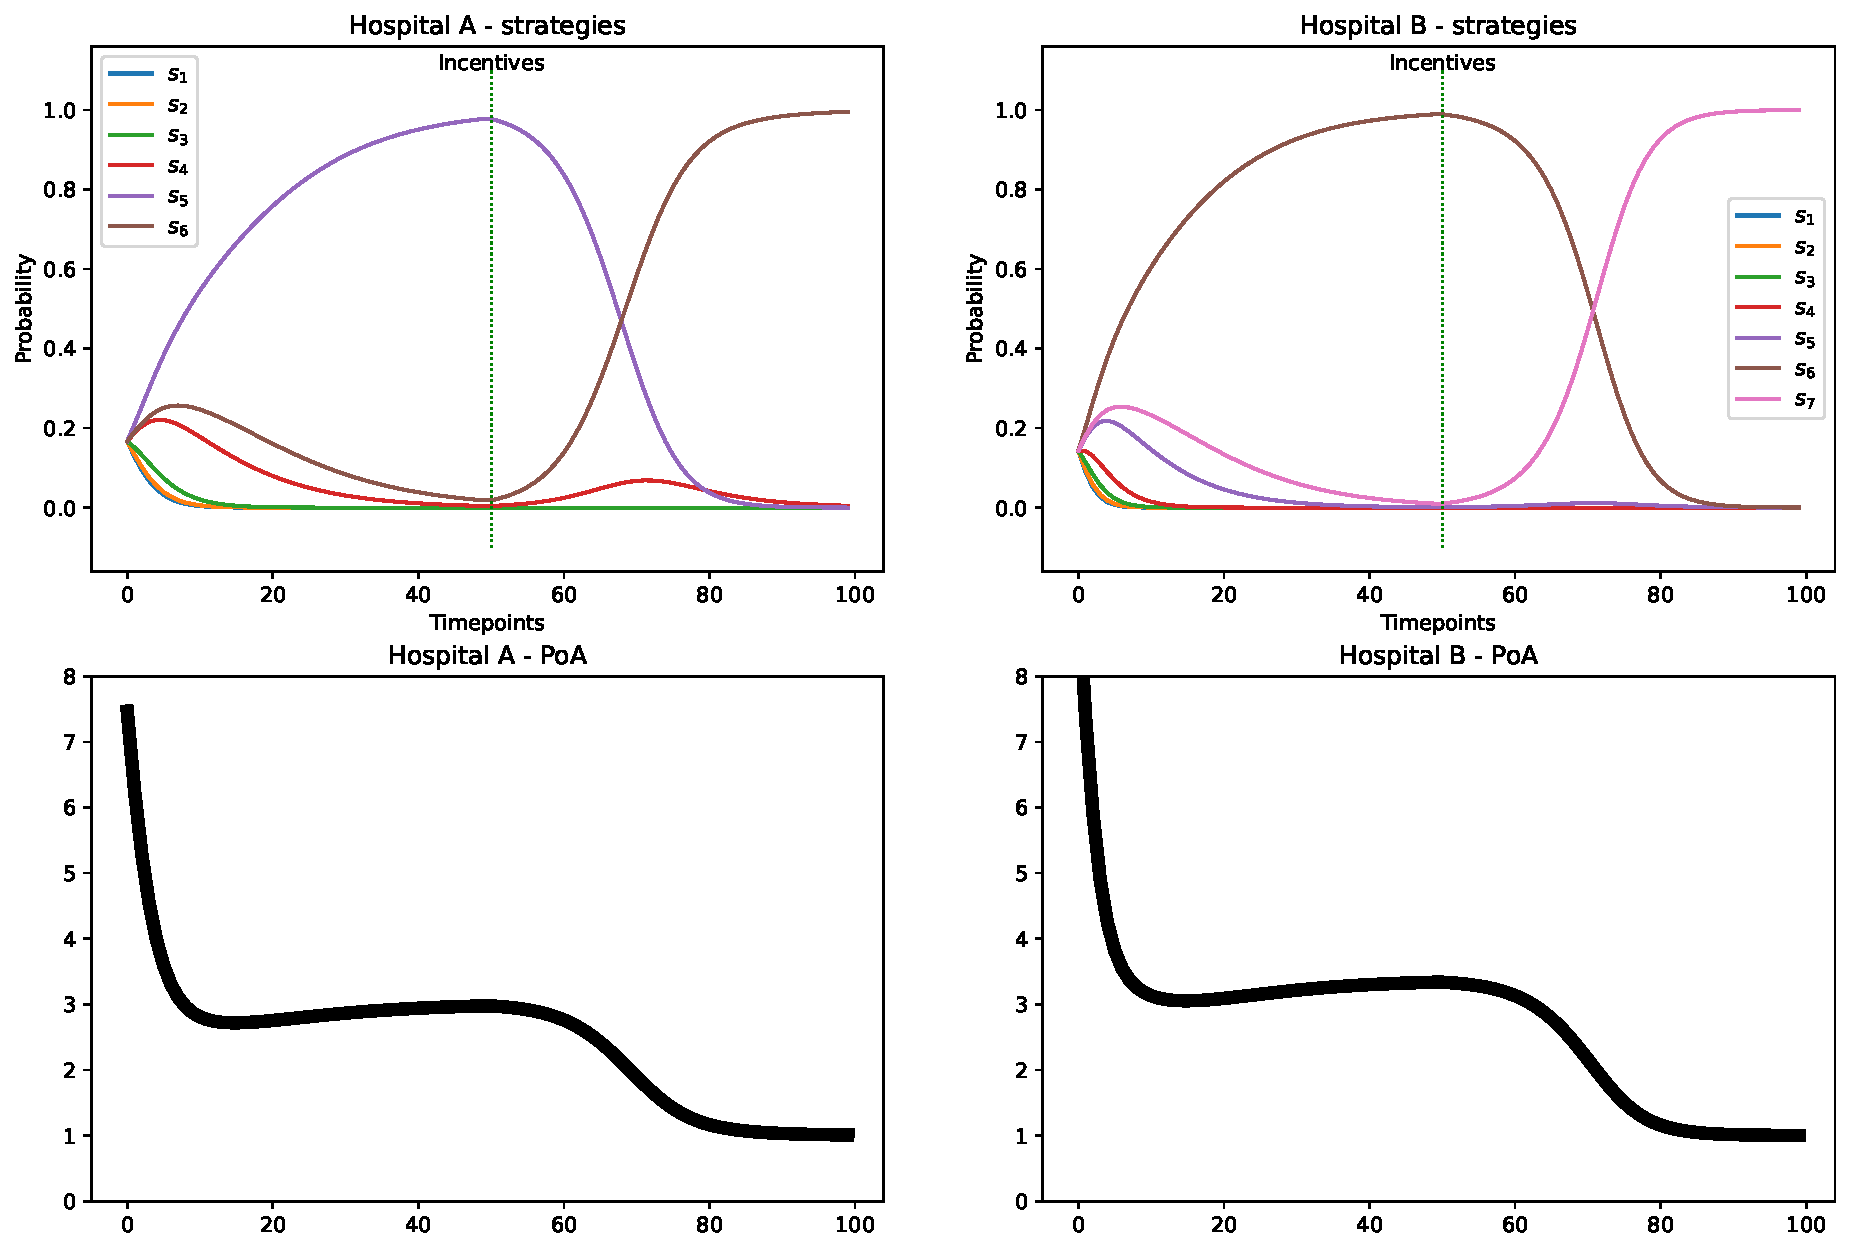
\includegraphics[width=\linewidth]{chapters/05_numerical_results/Bin/example_2/poa_ard_example_2_penalty.pdf}
    \caption{Example 2: Asymmetric replicator dynamics and compartmentalised
    \(PoA\) with incentivisation.}
    \label{fig:poa_ard_example_2_penalty}
\end{figure}

It can be seen that the hospitals start out by playing their usual strategies
of \(T^A = 5\) and \(T^B = 6\).
After the penalised matrices \(\tilde{A}\) and \(\tilde{B}\) are introduced,
the hospitals start to play strategies of \(T^A = 6\) and \(T^B = 7\).
That has a similar effect to the ones of
Figure~\ref{fig:poa_ard_example_2_num_of_servers} but no additional members of
staff have been added.
Additionally, the \(PoA\) for both hospitals is decreased, indicating that
the overall blocking time is reduced.

The results of this example show that using careful incentivisation on a
managerial level can result in an improvement of the overall blocking time
for the hospitals.
Although, arguably by adding more staff, the hospitals could have achieved
a greater reduction in the blocking time, these results indicate that when
that is not possible or not desirable, incentivisation can be used to
achieve a similar effect.

